% !TeX root = ../../main.tex
\section{Sensitivity analysis of KPIs}
\label{sec:sensitivities-kpis}
A sensitivity analysis on 5 key parameters was conducted to determine the robustness of Nitroma’s business plan and economic appraisal. NPV and payback period were selected as the KPIs for detailed analysis, whilst the results for IRR are summarised in Appendix XX. 

\subsection{Sensitivity to WACC}
% \begin{wrapfigure}{r}{8cm}
%     \vspace{-0.9cm}
%     \caption{Sensitivity of WACC on KPIs}
%     \label{Sensitivity_WACC}
%     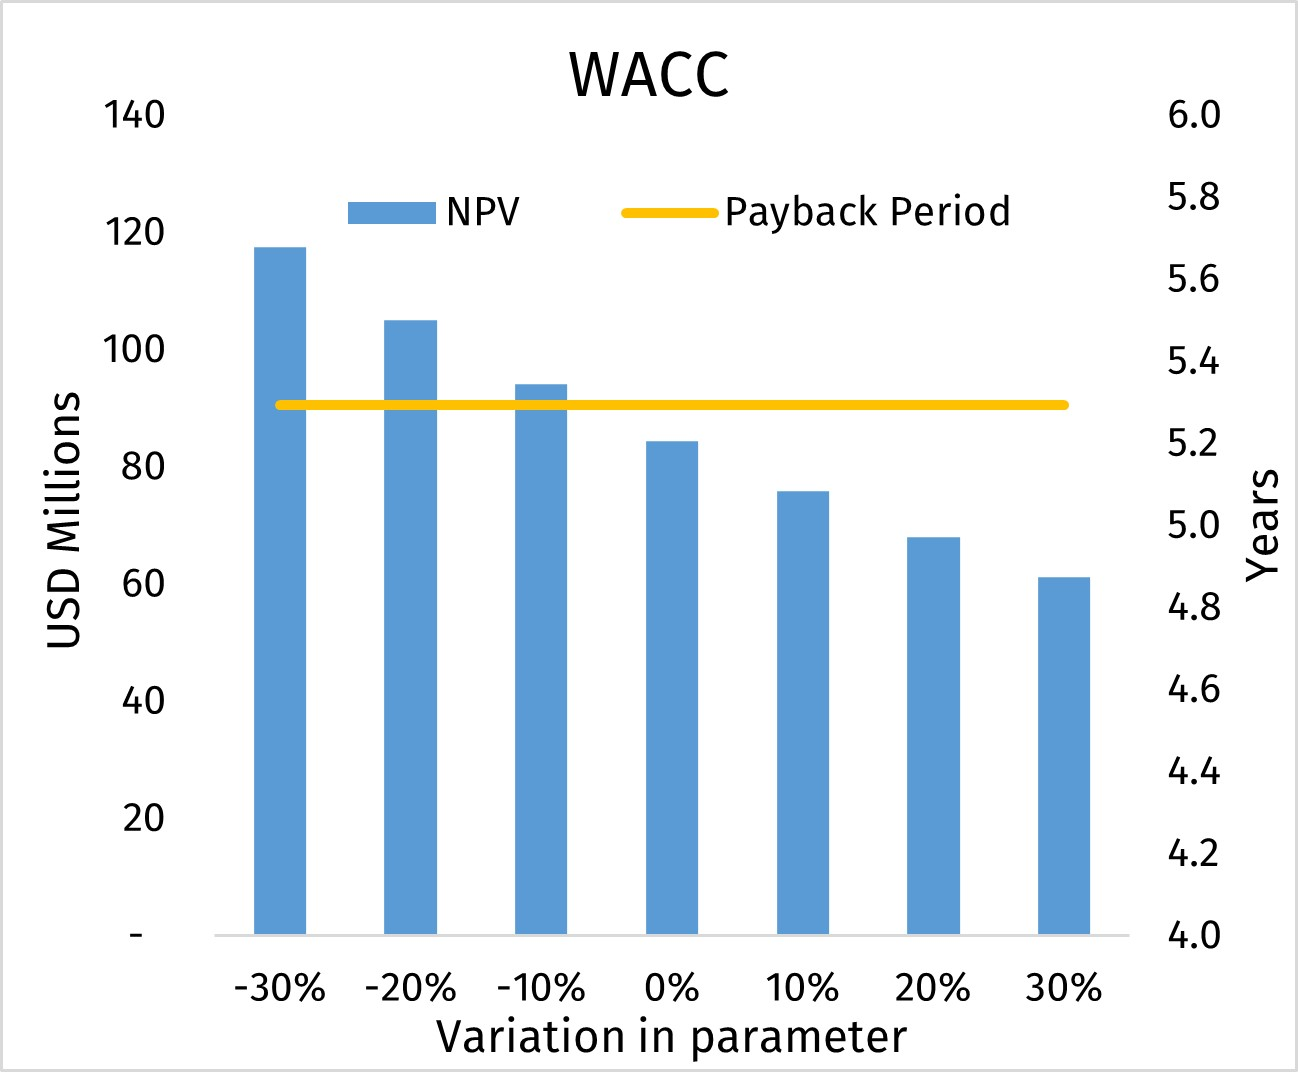
\includegraphics[width=0.47\textwidth]{chapters/6-economics/figures/Sensitivity_WACC.jpg}
% \end{wrapfigure}
WACC is an important variable because it considers the cost of equity, the cost of debt and corporate tax rate. Nitroma’s cost of equity may change if China’s risk-free rate changes – a likely scenario as China attempts to revive the economy following the coronavirus pandemic (XX). Similarly, the cost of debt may change depending on Nitroma’s creditworthiness.  Figure XX displays the effects of changing WACC on NPV and payback period. Even with a \SI{30}{\percent} increase in WACC, the project NPV decreased by roughly \SI{27}{\percent} to a healthy value of \$61.2 million. In fact, the WACC would need to increase by \SI{108}{\percent} for NPV to become negative - an unrealistic scenario. WACC does not affect payback period since payback period does not account for discounted cash flows, as discussed in \cref{sec:pby}. 
% As WACC increased, the NPV of the project decreased.

% \begin{figure}
% \centering
% \begin{minipage}{.5\textwidth}
%   \centering
%   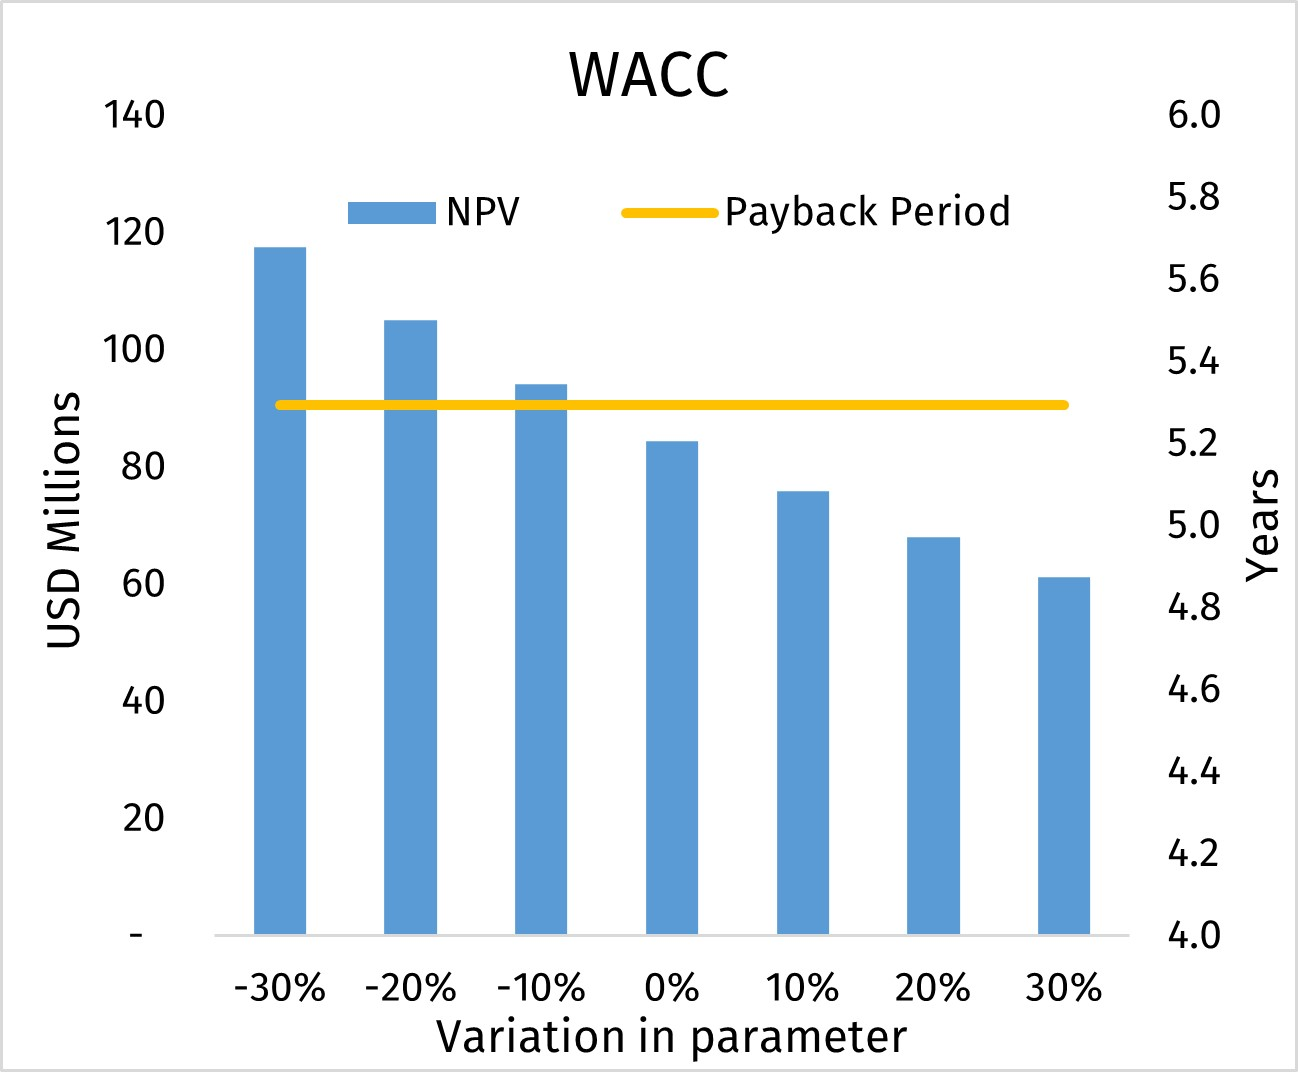
\includegraphics[width=0.95\textwidth]{chapters/6-economics/figures/Sensitivity_WACC.jpg}
%   \captionof{figure}{Sensitivity of WACC on KPIs}
%   \label{Sensitivity_WACC}
% \end{minipage}%
% \begin{minipage}{.5\textwidth}
%   \centering
%   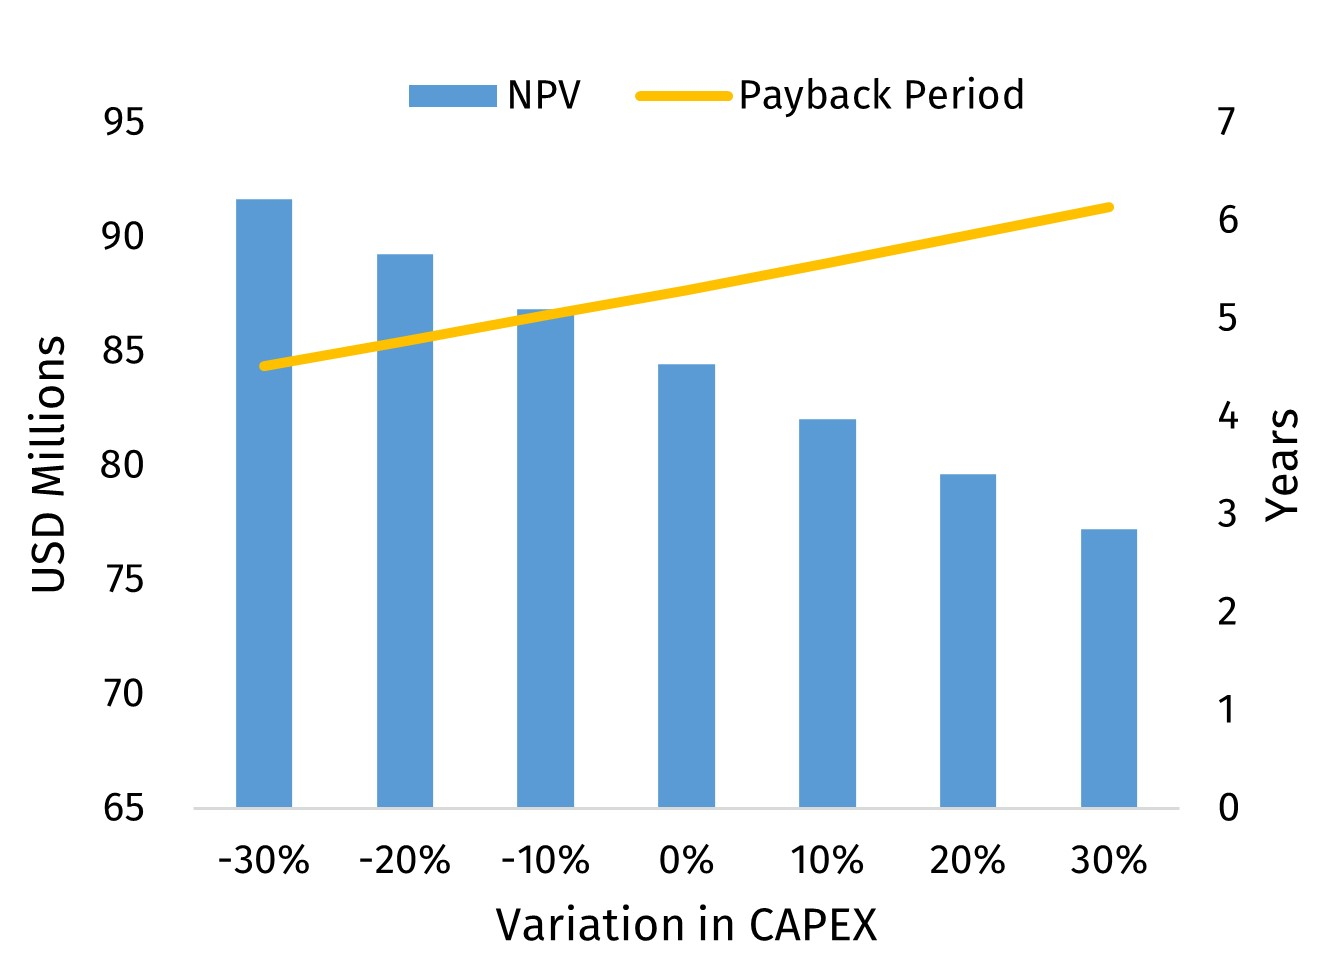
\includegraphics[width=0.95\textwidth]{chapters/6-economics/figures/Sensitivity_CAPEX.jpg}
%   \captionof{figure}{Sensitivity of CAPEX on KPIs}
%   \label{Sensitivity_CAPEX}
% \end{minipage}
% \end{figure}

\subsection{Sensitivity to CAPEX}
% \begin{wrapfigure}{r}{8cm}
%     \vspace{-0.9cm}
%     \caption{Sensitivity of CAPEX on KPIs}
%     \label{Sensitivity_CAPEX}
%     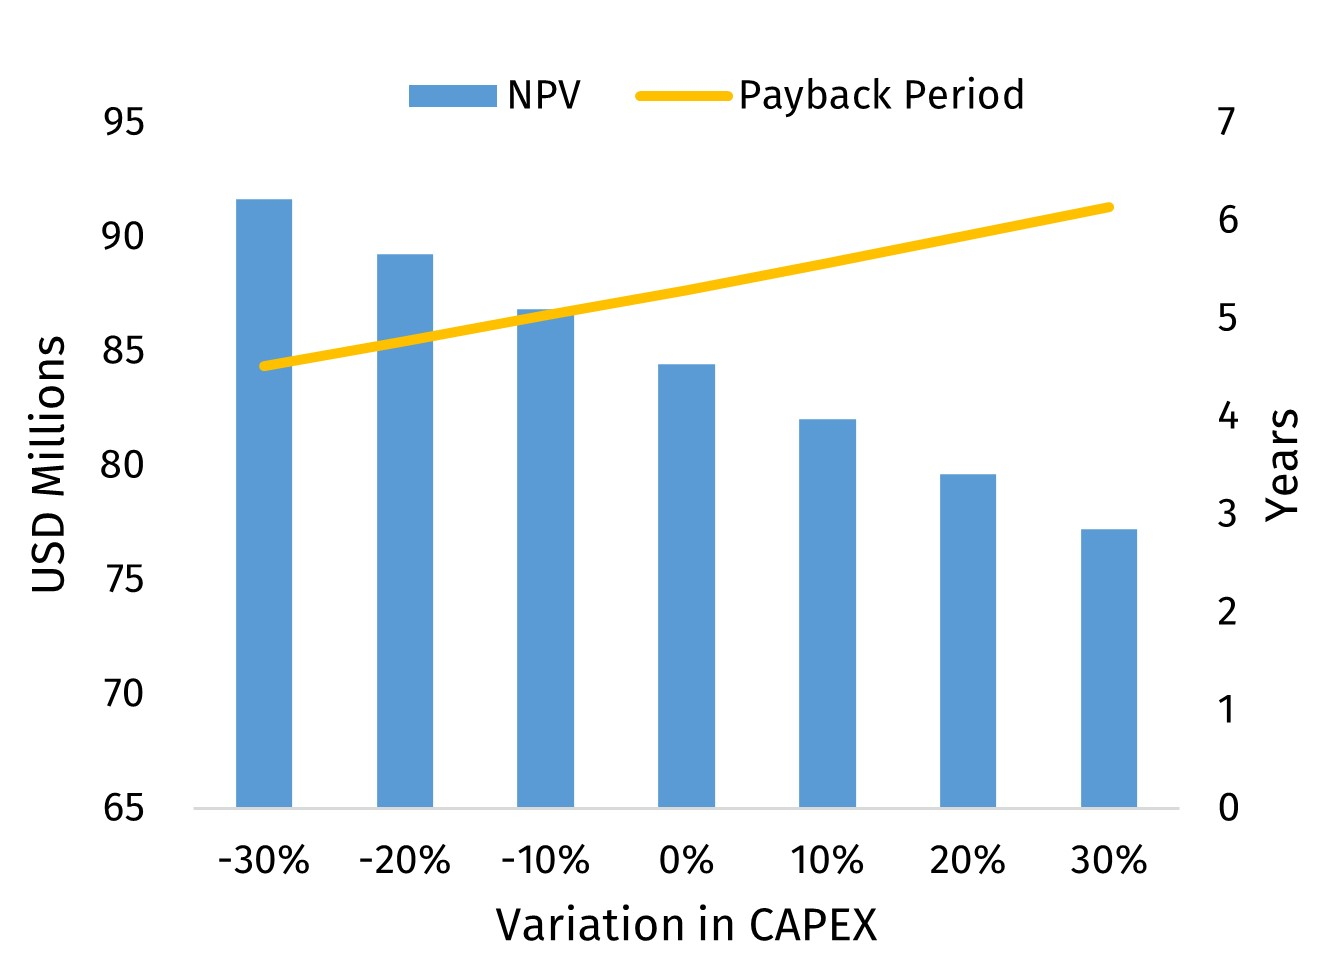
\includegraphics[width=0.47\textwidth]{chapters/6-economics/figures/Sensitivity_CAPEX.jpg}
% \end{wrapfigure}
Nitroma’s CAPEX was estimated using the methods suggested by Towler \& Sinnott, Douglas and Matche. Although these methods were averaged, CAPEX is a difficult value to project until direct quotes from manufacturers are obtained. Therefore, it important to conduct a sensitivity on this factor. As expected, CAPEX and NPV are inversely related. A \SI{30}{\percent} increase in CAPEX resulted in a \SI{9}{\percent} decrease in NPV to \$77.2 million and an increase in payback period to 6.1 years. It was found that CAPEX needs to increase 3.5x in order for the project NPV to become infeasible. This would be paired with an increase in payback period to 14.8 years – still less than the lifetime of the plant.

\subsection{Sensitivity to price of products}
% \begin{wrapfigure}{r}{8cm}
%     \vspace{-0.9cm}
%     \caption{Sensitivity of product prices on KPIs}
%     \label{Sensitivity_ProductPrice}
%     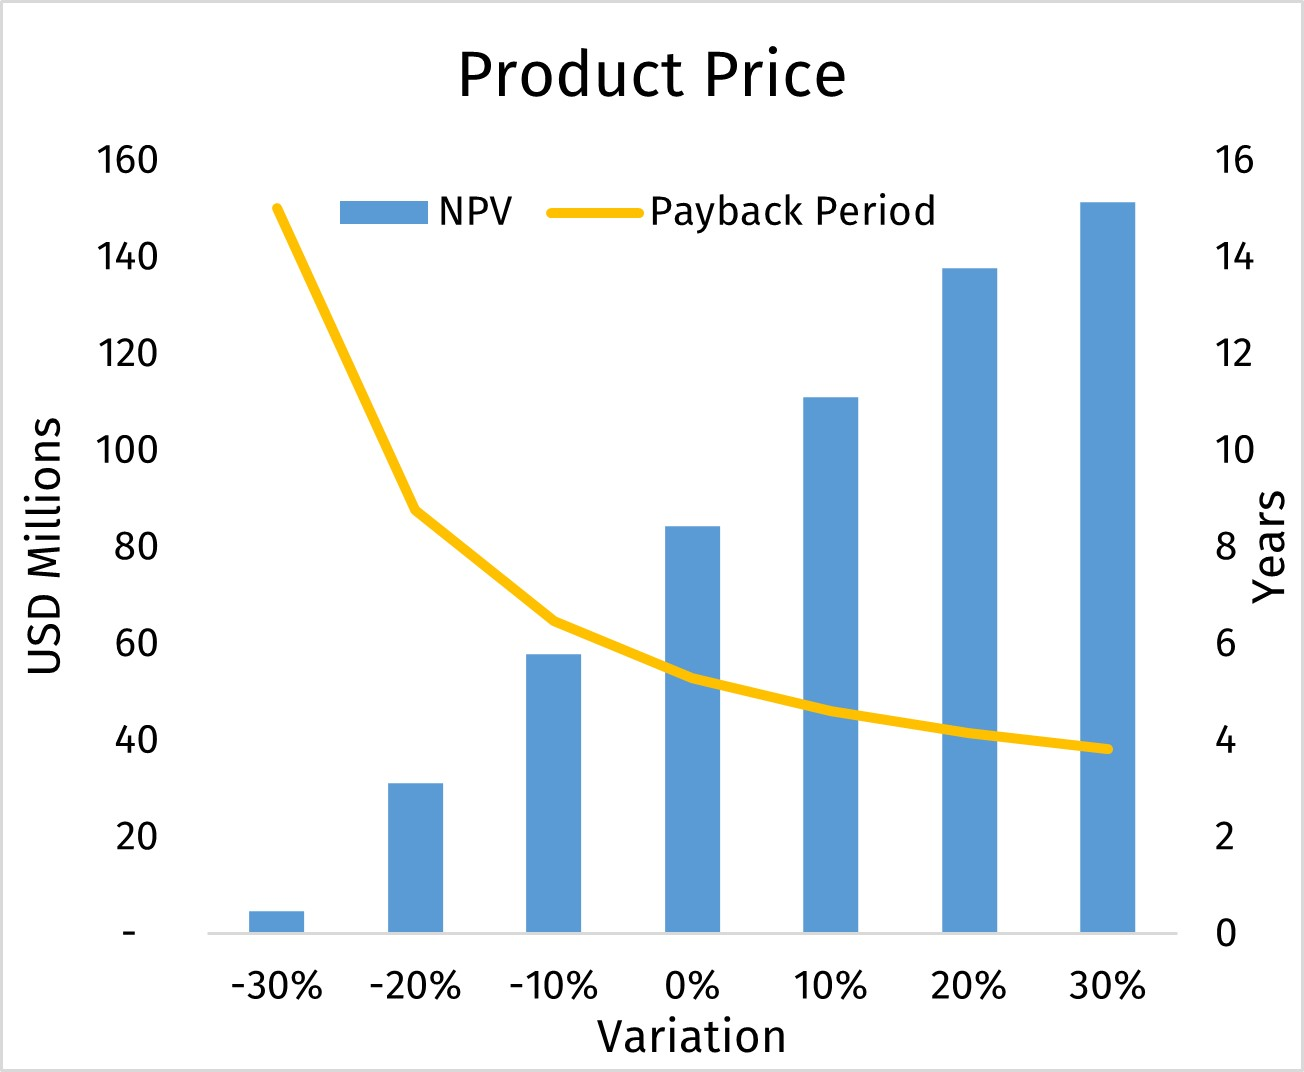
\includegraphics[width=0.47\textwidth]{chapters/6-economics/figures/Sensitivity_ProductPrice.jpg}
% \end{wrapfigure}
Nitroma’s revenue is entirely dependent on the price of its products, making it an important variable to test. It was found that a \SI{30}{\percent} decrease in product price resulted in NPV decreasing by \SI{95}{\percent} to \$4.6 million and the payback period increasing 3x to 15 years. Therefore, the feasibility of the project was deemed extremely sensitive to product price.  If the product price fell by \SI{33}{\percent}, the NPV became \$0. However, this scenario is unlikely as it implies a simultaneous price drop of \SI{33}{\percent} across all three of Nitroma’s products which are linked to three different industry sectors. Analyst forecasts have predicted strong growth for these sectors, as discussed in Section \ref{sec:market-analysis}, which should provide confidence to shareholders. In fact, the price of pain relief drugs like paracetamol increased by \SI{62}{\percent} following the pandemic which has a direct correlation with the price of PABA, a pain relief intermediate (XX).

\subsection{Sensitivity to plant commencement}
% \begin{wrapfigure}{r}{8cm}
%     \vspace{-0.9cm}
%     \caption{Sensitivity of plant commencement on KPIs}
%     \label{Sensitivity_ProductionDelay}
%     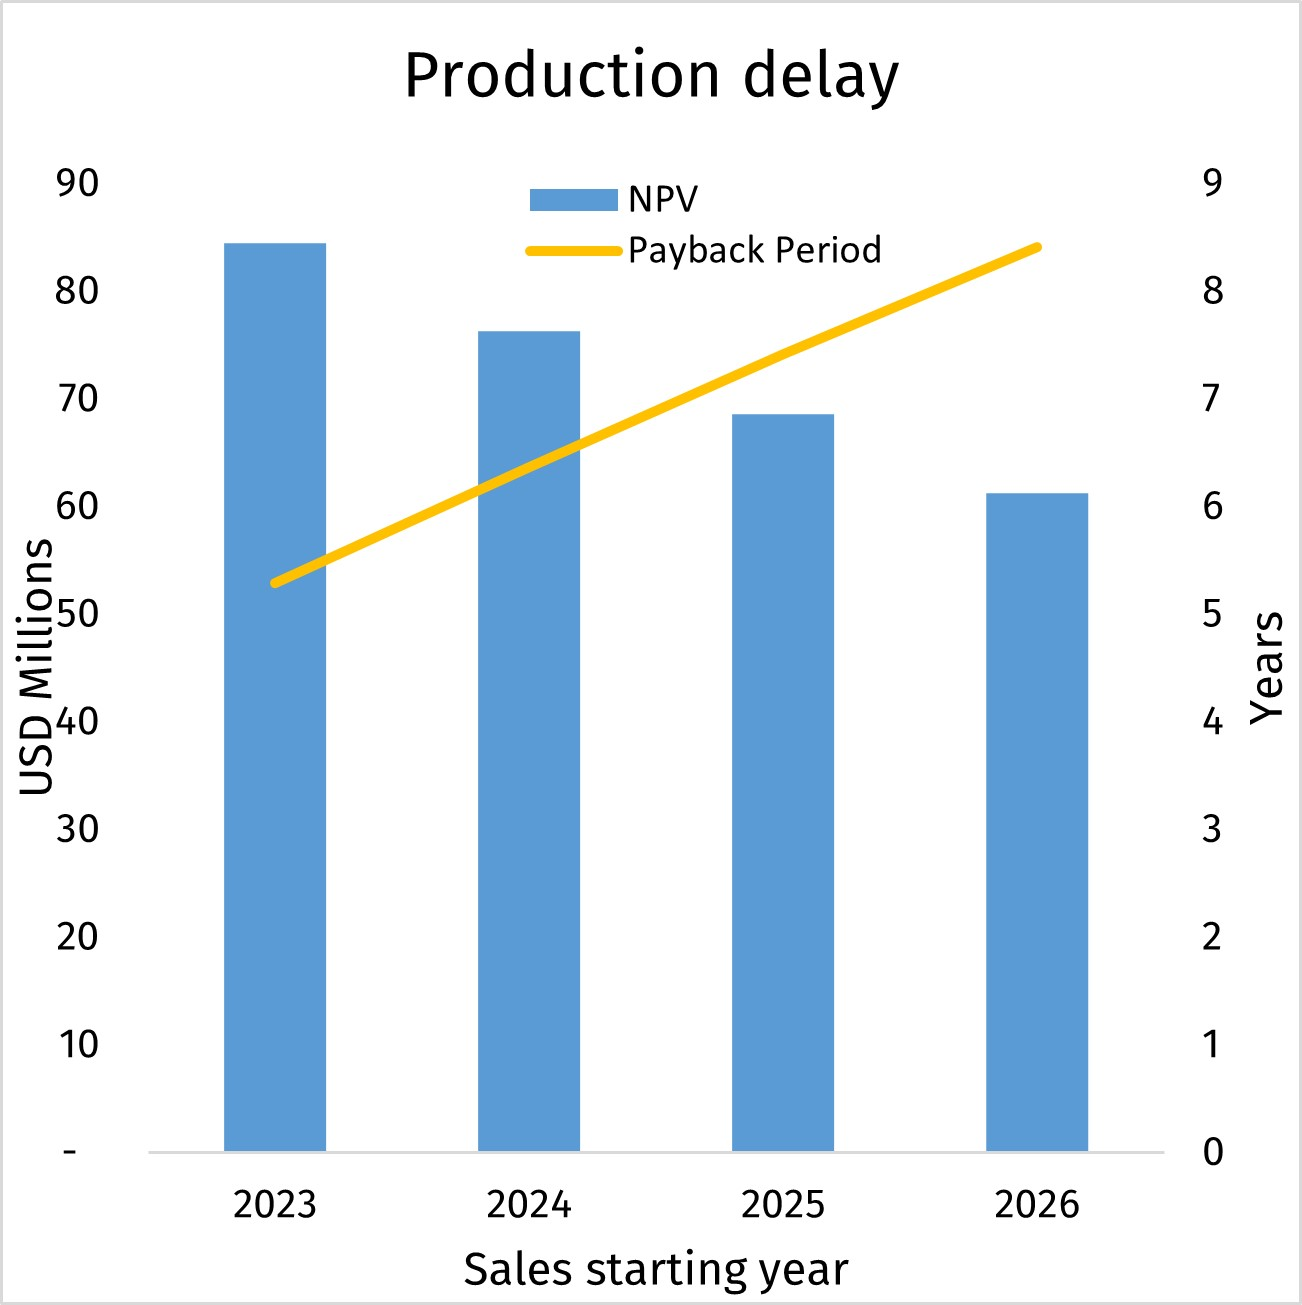
\includegraphics[width=0.47\textwidth]{chapters/6-economics/figures/Sensitivity_ProductionDelay.jpg}
% \end{wrapfigure}
Following the discussion in Section XX, it is important to test the feasibility of Nitroma’s business plan against a delay in production which is not unheard of in China. The importance of this parameter has been further highlighted by the coronavirus pandemic. Figure XX displays the sensitivity of NPV and payback period to the plant’s production date. A delay in sales \& distribution of even 3 years would result in a healthy NPV of \$61.2 million (\SI{27}{\percent} drop) and a payback period equal to industry average of 8.4 years. 

\subsection{Sensitivity to BH:BA days}
% \label{sec:sensitivity-ratiodays}
% \begin{wrapfigure}{r}{8cm}
%     \vspace{-0.9cm}
%     \caption{Sensitivity of BH:BA operating ays on KPIs}
%     \label{Sensitivity_BHBA}
%     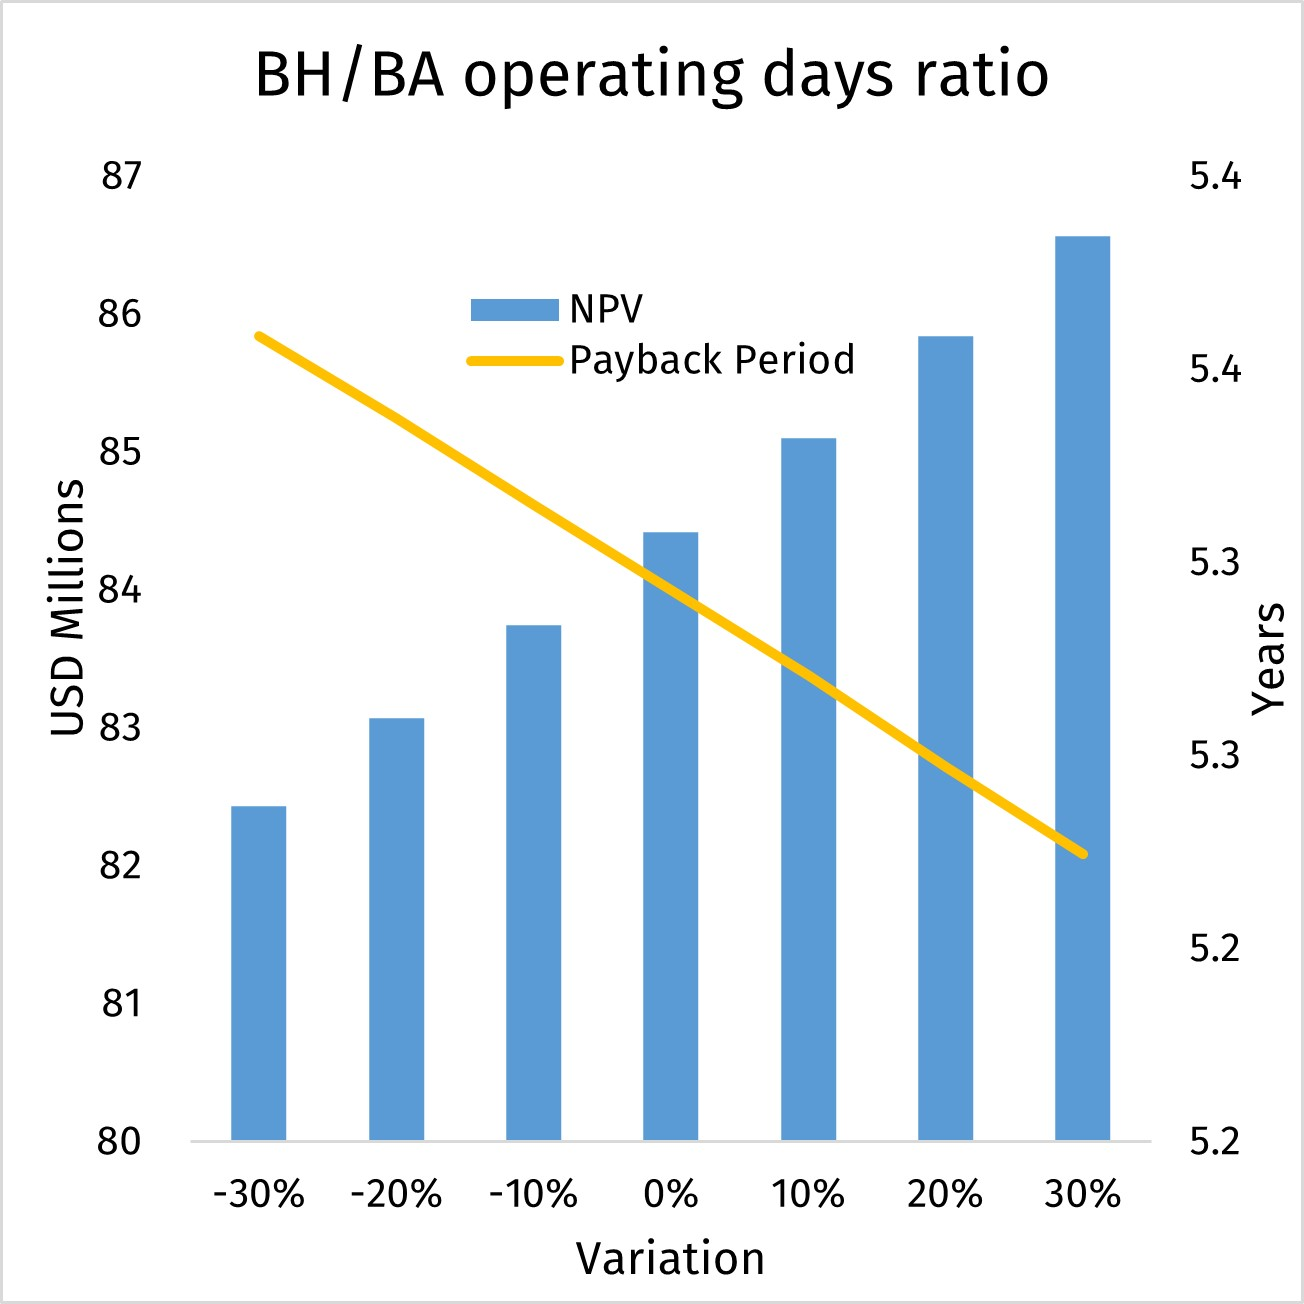
\includegraphics[width=0.47\textwidth]{chapters/6-economics/figures/Sensitivity_OperatingDays.jpg}
% \end{wrapfigure}
The ratio of days operating under BH production mode to days under BA production mode is an important factor that affects Nitroma’s profitability. If the ratio is increased by \SI{30}{\percent}, the project NPV increases by \SI{2.5}{\percent} and the payback period decreases by 0.1 years. Therefore, the feasibility of the project is minimally affected by a change in BH:BA. Plant modularity and a diverse product portfolio are key innovative features of Nitroma’s plant design, which offer the benefit of protection against market volatility. The current operational ratio has been carefully chosen to meet the domestic demand for each product (see \cref{sec:product-capacity}), but it is clear that changing this ratio due to fluctuating market demands does not affect the feasibility of Nitroma’s business.

% \begin{figure}
% \centering
% \begin{subfigure}[b]{.45\linewidth}
% 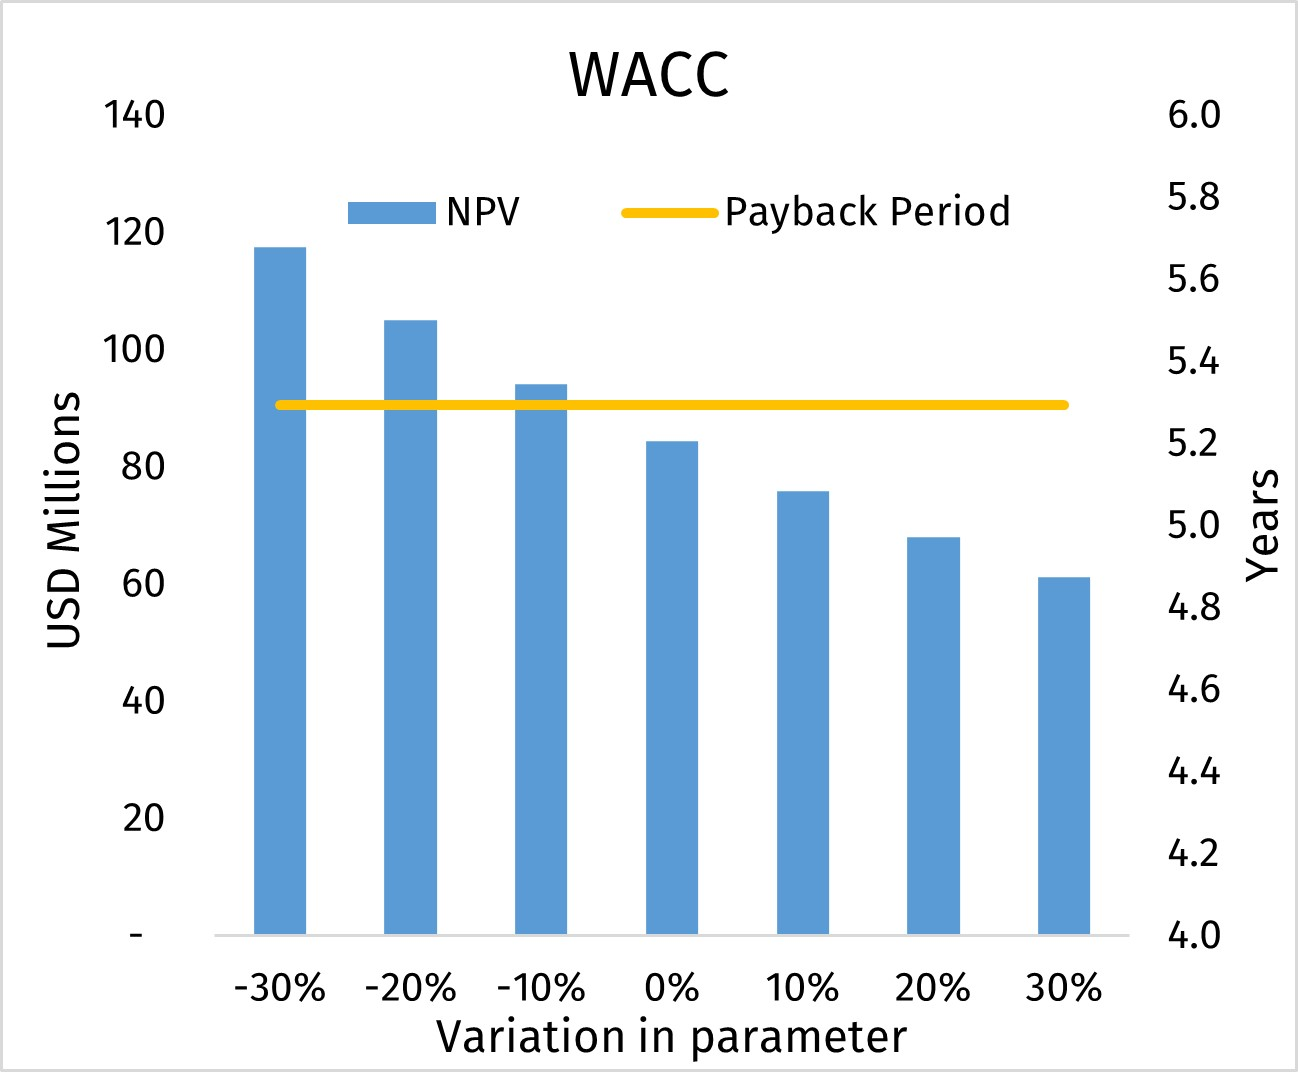
\includegraphics[width=\linewidth]{chapters/6-economics/figures/Sensitivity_WACC.jpg}
% \caption{Sensitivity of WACC on KPIs}\label{Sensitivity_WACC}
% \end{subfigure}

% \begin{subfigure}[b]{.45\linewidth}
% 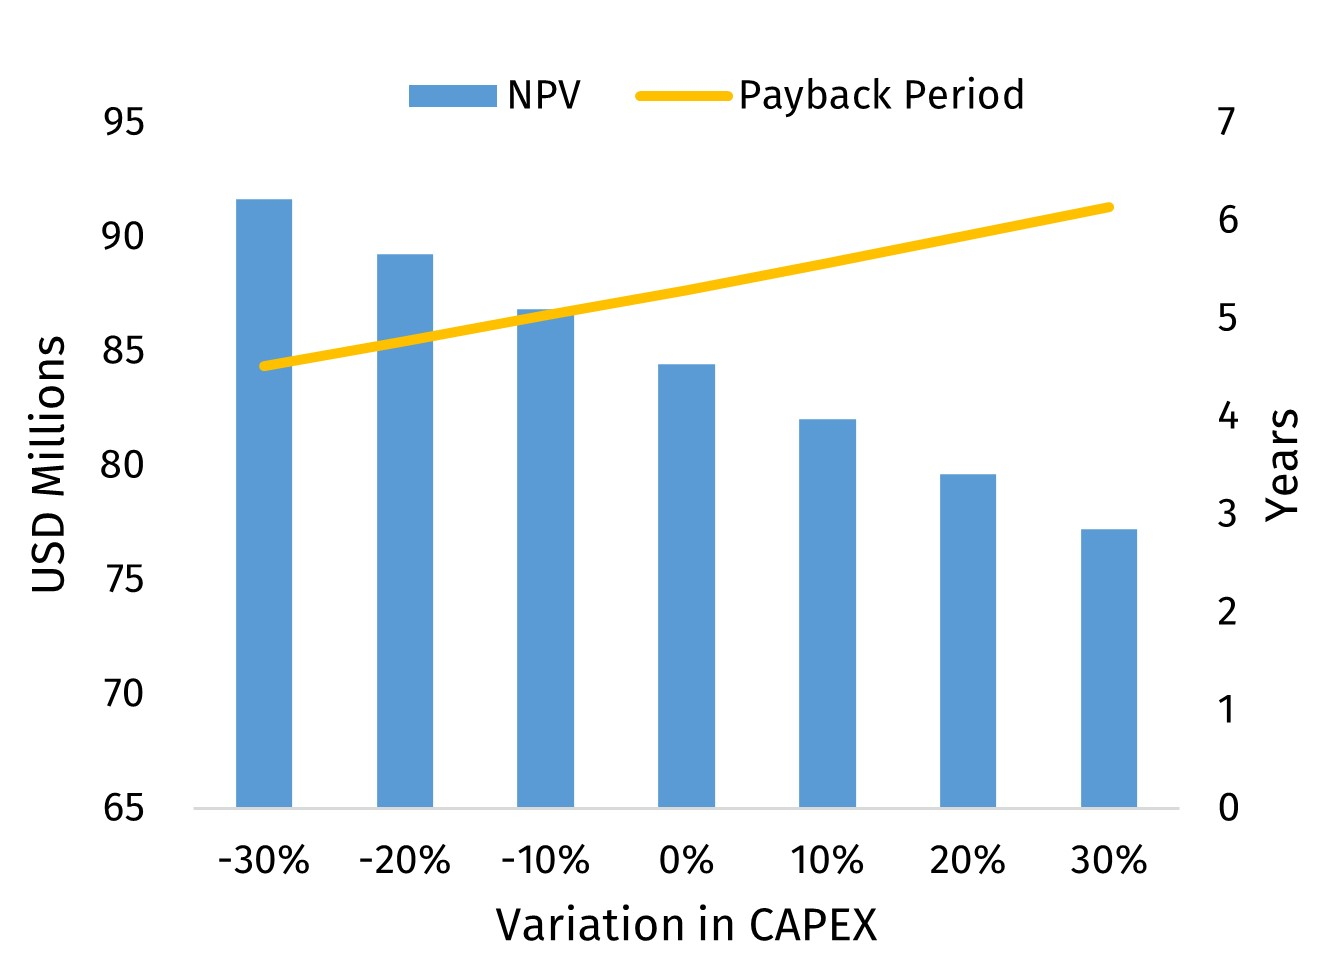
\includegraphics[width=\linewidth]{chapters/6-economics/figures/Sensitivity_CAPEX.jpg}
% \caption{Sensitivity of CAPEX on KPIs}\label{Sensitivity_CAPEX}
% \end{subfigure}
% \begin{subfigure}[b]{.45\linewidth}
% 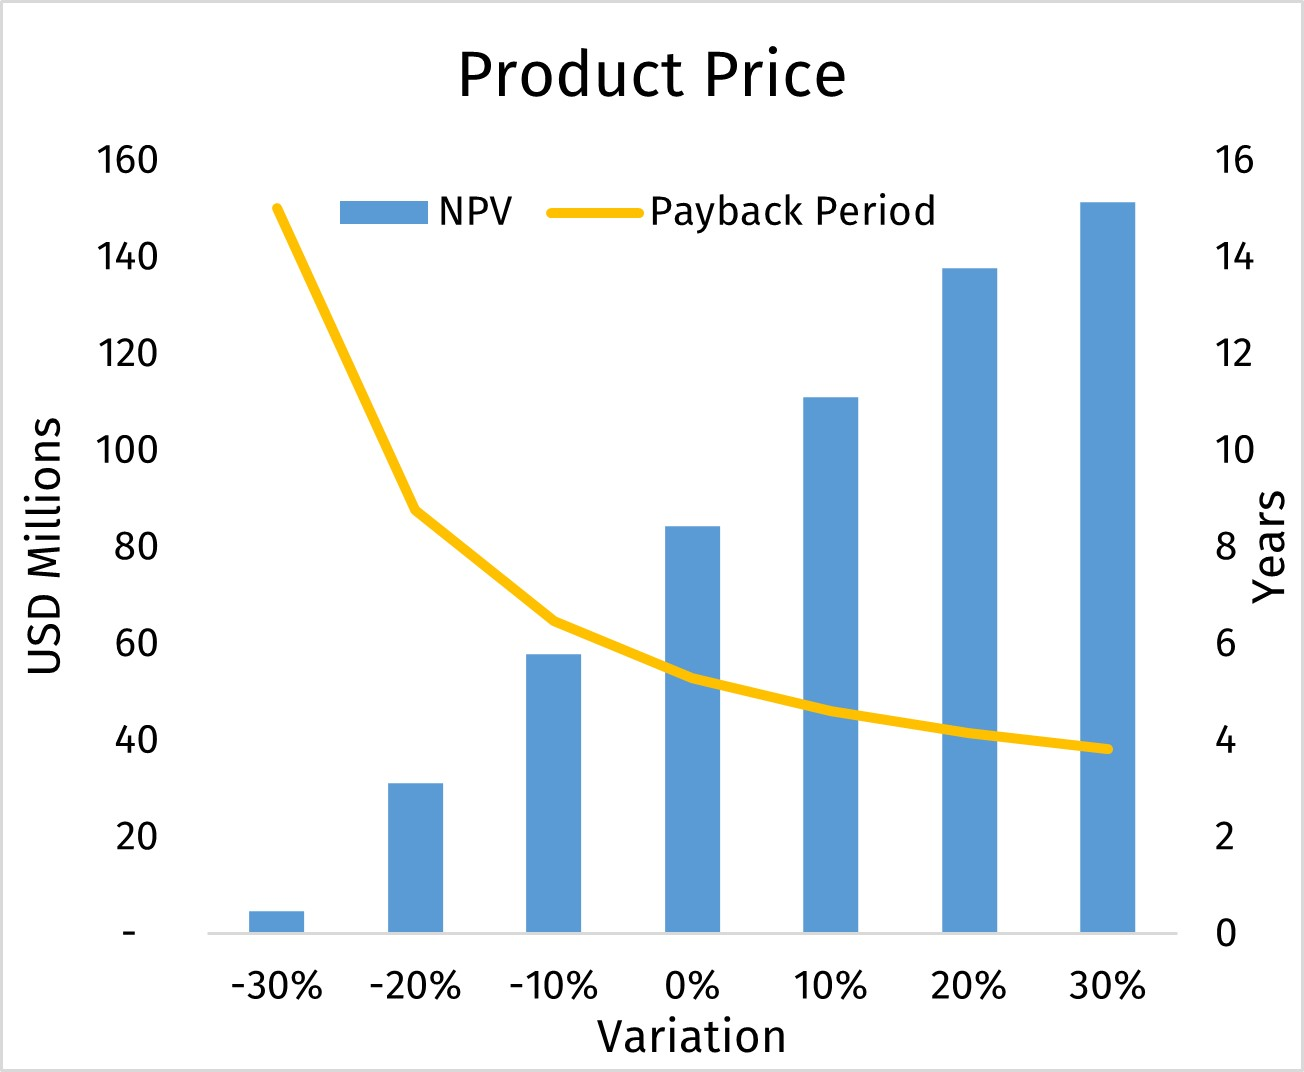
\includegraphics[width=\linewidth]{chapters/6-economics/figures/Sensitivity_ProductPrice.jpg}
% \caption{Sensitivity of product prices on KPIs}\label{Sensitivity_ProductPrice}
% \end{subfigure}
% \caption{Picture of animals}
% \label{Sensitivity_ProductPrice}
% \end{figure}

% \begin{wrapfigure}{r}{8cm}
%     \vspace{-0.9cm}
%     \caption{Sensitivity of product prices on KPIs}
%     \label{Sensitivity_ProductPrice}
%     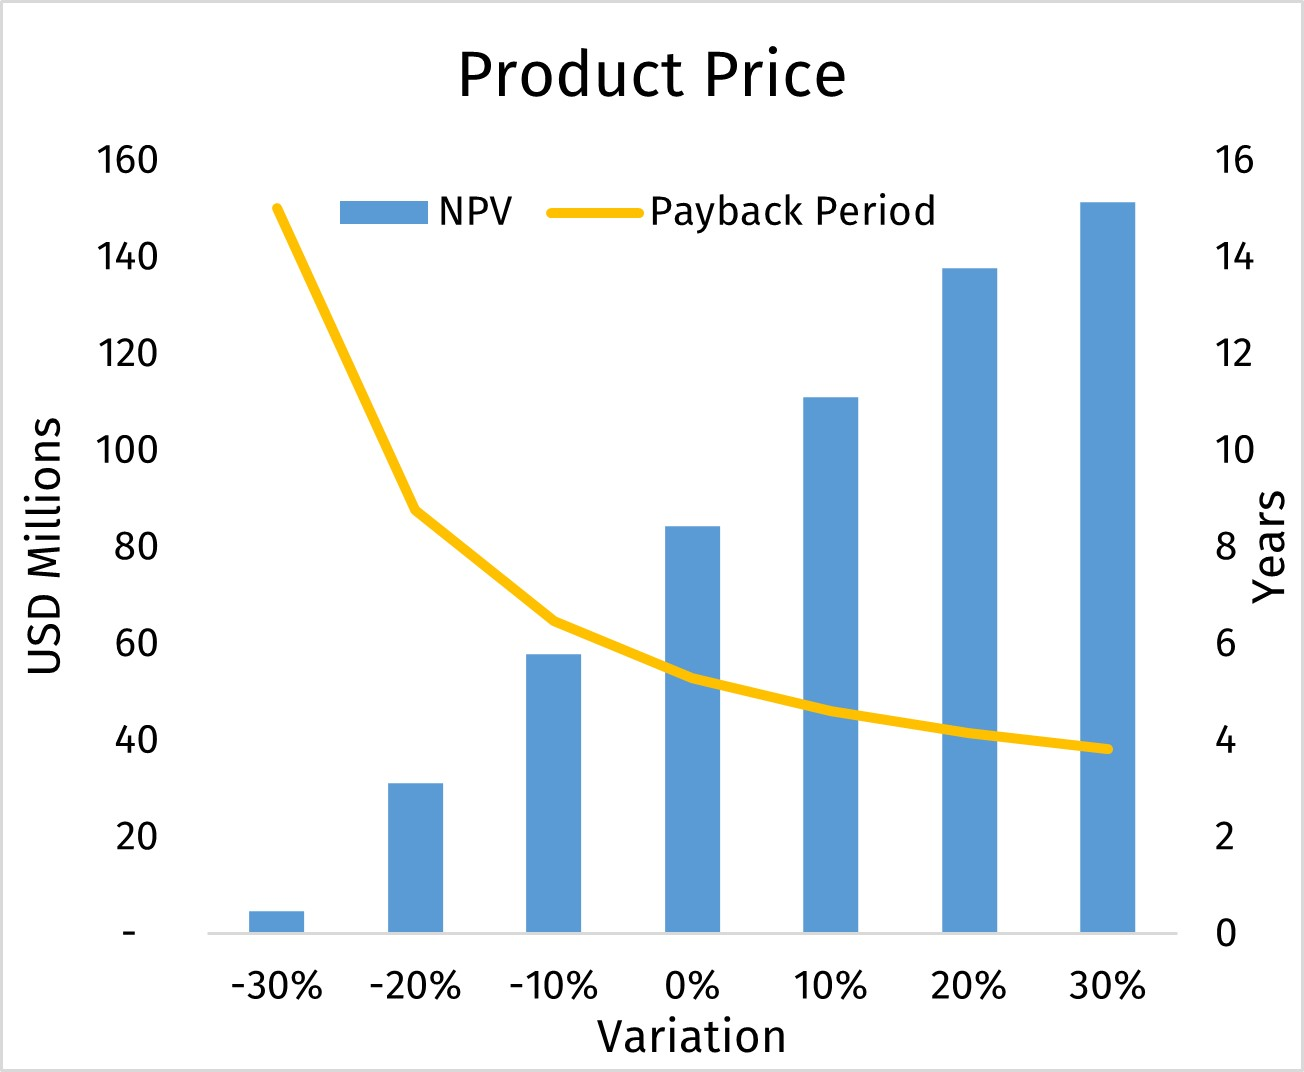
\includegraphics[width=0.47\textwidth]{chapters/6-economics/figures/Sensitivity_ProductPrice.jpg}
% \end{wrapfigure}